\documentclass{scrartcl}
\usepackage[utf8]{inputenc}
\usepackage[english]{babel}

\usepackage{amssymb,amsmath,amsthm}
\newtheorem{theorem}{Theorem}
\newtheorem{lemma}{Lemma}
\newtheorem{claim}{Lemma}
\theoremstyle{definition}
\newtheorem{definition}{Definition}[section]
\usepackage[bold]{hhtensor}


\usepackage{natbib}
\bibliographystyle{apalike}

\usepackage{hyperref}
\usepackage{cleveref}

\usepackage{todonotes}

\usepackage{booktabs}
\usepackage{float}

\DeclarePairedDelimiterX{\infdivx}[2]{(}{)}{%
  #1\;\delimsize\|\;#2%
}
\newcommand{\infdiv}{D\infdivx}

\DeclareMathOperator*{\cov}{cov}

\newcommand{\dd}{\mathrm{d}}

\newcommand{\cE}{\mathcal{E}}
\newcommand{\cL}{\mathcal{L}}
\newcommand{\cO}{\mathcal{O}}
\newcommand{\cP}{\mathcal{P}}
\newcommand{\cQ}{\mathcal{Q}}
\newcommand{\cS}{\mathcal{S}}

\newcommand{\eps}{\varepsilon}
\newcommand{\pd}{\partial}

\newcommand{\dist}{\mathrm{dist}}
\newcommand{\simiid}{\overset{\text{iid}}{\sim}}

\newcommand{\vb}{\vec{b}}
\newcommand{\vv}{\vec{v}}
\newcommand{\vx}{\vec{x}}
\newcommand{\vy}{\vec{y}}
\newcommand{\veta}{\vec{\eta}}

\newcommand{\mI}{\matr{I}}
\newcommand{\mM}{\matr{M}}

\newcommand{\RR}{\mathbb{R}}
\newcommand{\EE}{\mathbb{E}}
\newcommand{\PP}{\mathbb{P}}

\newcommand{\cN}{\mathcal{N}}

\newcommand{\feynman}[1]{{\color{blue}{(Feynman: {#1})}}}
\newcommand{\liam}[1]{{\color{green}{(Liam: {#1})}}}
\newcommand{\michael}[1]{{\color{purple}{(Michael: {#1})}}}


\title{Fat-Tailed Variational Inference}

\begin{document}
\maketitle

Given a probabilistic model $p(x,y)$, the goal of automatic variational
inference is to (1) construct a variational family of distributions
$\{q_\phi\}_{\phi \in \Phi}$ and (2) search for a good variational
approximation to the posterior $q_\phi \approx p(x \mid y)$.
We focus on (1) and consider variational families specifically constructed
to include fat-tailed members. Our contributions:
\begin{enumerate}
    \item We rectify the failure of ADVI against fat tailed target densities by
          extending it to utilize Student-T variational family, and extend its
          applicability by transforming the density through a normalizing flow
          analogous to \citep{webb2019improving}.
          Our results on a location-scale representation for a StudentT shows that (1)
          allowing users to specify a tail-index for variational approximators leads to
          better fits and (2) even without prior knowledge, estimating the tail
          coefficient during training also works.
    \item We provide alternatives for estimation of the variational
          approximation's tail index, adapting ideas from classical tail index
          estimation (\cite{hill1975simple,pickands1975statistical}) to the
          variational inference setting where posterior samples are expensive but
          joint log density evaluations are cheap
\end{enumerate}

\section{Background}

Probabilistic machine learning problems are coveniently formalized using
probabilistic programming languages (PPLs) which provide high level
primitives for probabilistic modelling and inference. In order to enable more
flexibile and precise control over variational inference methods, recent work
has explored a design space for variational inference APIs ranging from
limited but completely automated (ADVI, \cite{kucukelbir2017automatic}) to
manually specified guide programs (WebPPL, Pyro). Our work here focuses on
automated variational inference where we seek to automatically construct a
reasonable variational family automatically after tracing the execution of
the probabilistic program.

Fat-tailed distributions commonly arise in robust machine learning where a
standard approach is to replace light-tailed noise distributions fat-tailed
ones \cite{tipping2005variational}. They are also commonly used as weakly
informative prior distributions in Bayesian heirarchical models
\cite{gelman2006prior}.

\subsection{Related Work}

The Box-Cox transform \citep{box1964analysis} is a commonly used parametric
power transform to address fat tails and make data more similar to a normal
distribution. This is analogous to composing a power transform before
the normalizing flow. Whereas \cite{asar2017estimating} fit this transform
using goodness-of-fit tests against a normal, whereas our optimization signal
is back-propagated from an ELBO against the target posterior.

The bulk of related work focuses on fat-tails arising from relaxing priors.
Recent work in VAEs has extensively studied the impact of relaxing Gaussian
assumptions to heavier-tailed distributions. \citep{mathieu2019disentangling}
consider a StudentT prior distribution $p(z)$ over the latent code $z$ in a
VAE with Gaussian encoder $q(z \mid x)$
\footnote{\url{https://github.com/iffsid/disentangling-disentanglement/blob/3396d40f46c34dd928a1241f567a86276b0ff41b/src/main.py\#L52}},
showing that the anisotropy of a StudentT product distribution (compared to
the standard choice of Normal prior) leads to more disentangled
representations. \cite{chen2020use} perform a similar modification except in
a coupled VAE \cite{cao2019coupled} and showed improvements in the marginal
likelihoods of reconstructed images. In addition,
\cite{boenninghoff2020variational} consider a mixture of StudentTs for the
prior $p(z)$. Finally, \feynman{maybe remove this? it was rejected from
    ICLR}, \cite{abiri2020variational} considered both StudentT prior and
variational approximation family and showed improvements in SSIM (structural
similarity) score of between original and reconstructed images. To position
our work in context, note that the VAE's encoder $q(z \mid x)$ may be viewed
as a variational approximation to the posterior $p(z \mid x)$ defined by the
decoder model $p(x \mid z)$ and the prior $p(z)$. Our work differs from
\citep{mathieu2019disentangling,chen2020use,boenninghoff2020variational} in
that we consider heavy-tailed variational approximations $q(z \mid x)$ rather
than priors $p(z)$, and although \citep{abiri2020variational} also considers
a StudentT approximate posterior our work (1) considers a more general
variational family comprised of flow transforms of StudentTs and (2) conducts
a more thorough investigation across a broader range of models beyond a VAE
on FashionMNIST.

Relaxation of priors to heavy-tailed distributions has numerous
applications beyond VAEs. In \cite{silnova2018fast}, the authors perform
inference in heavy-tailed probabilistic linear discriminant analysis
using Gaussian mean-field variational inference and show improved
accuracy in speaker identification. Our work is complementary to these approaches;
whereas they consider heavy-tailed priors $p(z)$ we consider heavy-tailed
variational families $q(z \mid x)$.

More directly comparable recent work on fat-tailed variational families
\cite{ding2011t,futami2017expectation} studies the $t$-exponential family
variational approximation (which includes Student-Ts and other
heavier-tailed) includes heavy-tailed variational families, but critically do
not discuss selection of the parameter $t$ (which is deterministically to the
Student-T's DoF $v$). Other differences include their derivation of
expectation propagation update equations whereas we directly backprop a noisy
ELBO estimate, and our broader variational family which includes flow
transforms.

Most related to our work is \cite{jaini2020tails}, which shows similar
impossibility results with Gaussian tailed base distributions and consider
flow transforms of StudentT base distributions. However, our tail adaptive
flows (1) do not mandate equal tail index across all dimensions, (2) composes
techniques from \cite{kucukelbir2017automatic} to address target
distributions with constrained support, (3) are investigated within the
setting of density estimatino ($\propto KL(p,q)$, test set likelihood) as
variational inference ($KL(q,p)$, ELBO, since $p$ is a posterior hard to
sample), and (4) are automatically generated as part of a probabilistic
programming engine.

\section{Fat Tailed Variational Inference}

\subsection{Distribution classes}

While there is significant attention on parameterizing the transport map, there is comparatively little interest in considering the distribution $p$ of the latent variable $Z$. Because the vast majority of transport map parameterizations are Lipschitz continuous, we will find that this choice of $p$ can have a profound impact on the quality of the approximation of the tails of the target distribution. Here, we shall consider the following three main types of tail behaviour.
\begin{enumerate}
    \item The class $\mathcal{G}$ of subgaussian random vectors $X$ satisfying \[\limsup_{r\to\infty}r^{-2}\log\mathbb{P}(\|X\|>r)<0.\]
    \item The class $\mathcal{E}$ of subexponential random vectors $X$ satisfying \[\limsup_{r\to\infty}r^{-1}\log\mathbb{P}(\|X\|>r)<0.\]
    \item The class $\mathcal{P}_\nu$ of random vectors $X$ with tails no heavier than a $\nu$-power law, that is, \[\limsup_{r\to\infty}\log\mathbb{P}(\|X\|>r)/\log r<-\nu.\]
\end{enumerate}
It is more convenient to characterize these distribution classes according to the concentration function $\alpha_X$ defined for a random vector $X$ by
\[
    \alpha_{X}(r)=\sup_{A\,:\,\mathbb{P}(X\in A)\geq1/2}\mathbb{P}(\mbox{dist}(X,A)>r),
\]
where $\dist(x,A) = \inf_{y \in A}\|x - y\|$. Equivalent characterizations of $\mathcal{G},\mathcal{E},\mathcal{P}_\nu$ follow by replacing $\mathbb{P}(\|X\|>r)$ with $\alpha_X(r)$. For example, a random variable $X \in \mathcal{G}$ if and only if $\limsup_{r\to\infty} r^{-2} \alpha_X(r) < 0$. Under this observation, the following lemma is an immediate consequence of \cite[Proposition 1.3]{ledoux2001concentration}.
\begin{lemma}
    \label{lem:distn_class_closed}
    The classes $\mathcal{G}$, $\mathcal{E}$, and $\mathcal{P}_\nu$ for any $\nu > 0$, are closed under Lipschitz transformations. In other words, if $f$ is Lipschitz, then for any $X \in \mathcal{G}$ (resp. $\mathcal{E}$, $\mathcal{P}_\nu$), $f(X) \in \mathcal{G}$ (resp. $\mathcal{E}$, $\mathcal{P}_\nu$). 
\end{lemma}
In other words, using only transport map approximators based on Lipschitz transformations, to achieve an accurate approximation of the tails of the target distribution, one must ensure that the reference distribution exhibits the same tail behaviour. Density estimators using a base distribution of incorrect class will inevitably fail at approximating slower tail decay. Note that this is not in violation of universal approximation theory since $\mathcal{G}$ is dense in $L^{2}$ (and therefore in $\mathcal{E}$ and $\bigcup_{\nu>0}\mathcal{P}_{\nu}$). 

Two noteworthy choices for $p$ in the literature are the standard Gaussian distribution, as seen in  \cite{kingma2016improved}, and the logistic distribution, as seen in \cite{dinh2014nice} (recommended because it ``tends to provide a better behaved gradient''). Indeed, in the former case, only subgaussian approximations are available. In the latter case, since the logistic distribution is subexponential and not subgaussian, subexponential approximations are available. However, neither of these choices are effective for distributions which exhibit power-law tails, such as the Student $t$-distribution. 


\feynman{From 1/29/2021:
    
    New theory? Extend multivariate reuslts of \cite{jaini2020tails} to invalidate shared $\nu$, eg 
    product of two studentT with very different DoF.
    Interaction between ADVI transformed distributions and StudentTs.
    
}

\subsection{Fat tails and tail indices}
\feynman{Reconcile with distribution classes}

\begin{definition}[\cite{resnick2007heavy}]
    A random variable $X$ has \emph{fat tails} with
    tail index $\alpha > 0$
    if $\Pr[X > x] \sim x^{-\alpha}$ as $x \to \infty$.
\end{definition}

Variance undefined if $\alpha < 3$, generally all moments $> \alpha - 1$
are infinite. $\alpha$ is called the \emph{tail index}.

Can relax power law to regularly/slowly varying \footnote{\url{https://journals.aps.org/prresearch/abstract/10.1103/PhysRevResearch.1.033034}}, which permits deviations without
affecting tail exponent.

Pareto: $\Pr[X > x] = \left(\frac{x_m}{x}\right)^\alpha \sim x^{-\alpha}$

Student T \footnote{\url{https://math.stackexchange.com/questions/3092190/asymptotics-of-hypergeometric-2f-1abcz-for-large-z-to-infty}}: 
$\Pr[X > x] \sim x \left(\frac{x^2}{\nu}\right)^{-\frac{1}{2}} + \left(\frac{x^2}{\nu}\right)^{-\frac{\nu+1}{2}} \sim x^{-\nu}$.

Cauchy: $\Pr[X > x] \sim -\arctan\left(\frac{x - x_0}{\gamma}\right) \sim x^{-1}$,
which makes since because standard Cauchy is StudentT($\nu=1$).

Stable distributions? $X$ is stable if $\forall a, b > 0$, 
$a X_1 + b X_2 = c X + d$ for some $c > 0$, $d$ where $X_1, X_2$ independent copies of $X$
(closure under convolution for fixed $\alpha$).
This includes normal, Cauchy, and Levy. Four parameter family with stability parameter $\alpha$
controlling the asymptotic behavior (tail index?). $\alpha = 2$ gives a Guassian,
and $\alpha < 2$ gives $p(x) \sim \lvert x \rvert^{-(\alpha + 1)}$.

\feynman{Reconcile definitions with \cite{jaini2020tails}}

\subsection{Flows in variational inference}

Universal approximation theorems about flows are not violated; they are asymptotic
so finite realizations will still have support $\RR$ and Lipschitz continuity.

\textbf{IMPORTANT}: support $\RR$ makes them unsuitable for VI's $KL(q,p)$, need \cite{kucukelbir2017automatic}
transforms

\subsection{Failure modes on fat-tailed target densities}
\label{ssec:failure}

One major limitation of $p = N(0,I)$ is:
\begin{theorem}[Chapter 2 \cite{wainwright2019high}]
    Let $(X_i)_1^n$ be a vector of iid $N(0,1)$ RVs,
    $f : \RR^n \to \RR$ be $L$-Lipschitz.
    Then $f(X) - \EE f(X)$ is $L$-sub-Gaussian.
\end{theorem}
In particular, density estimators using a Gaussian base
distribution $p$ will inevitably fail at approximating slower
tail decay.

When the target density is a fat-tailed Cauchy distribution as in
\cref{fig:cauchy_normal_student}, variational inference using
flow-transformed Gaussian base distributions \cite{webb2019improving} (orange
in left) result in tails which decay inappropriately fast as measured
using a Kolmogorov-Smirnov goodness-of-fit test (right). In contrast,
the learned flow-transformed Student-T base distribution (green left)
provides a much better approximation of the tail behavior.

\begin{figure}[H]
    \centering
    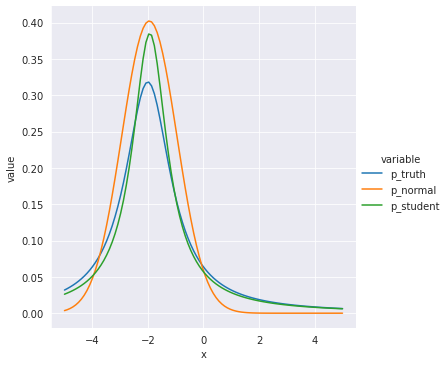
\includegraphics[width=0.49\textwidth]{Figures/cauchy_normal_student.png}
    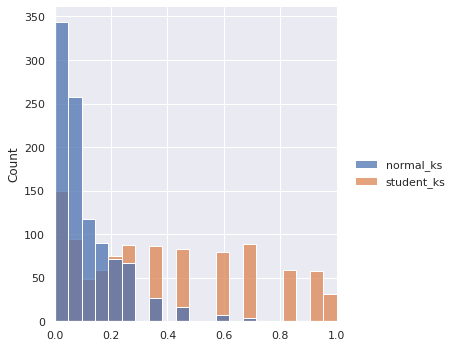
\includegraphics[width=0.49\textwidth]{Figures/cauchy_ks.png}
    \caption{VI against a Cauchy target, PDFs (left) and $p$-value of Kolmogorov-Smirnov test statistics (right, $\leq 0.05$
        suggests poor approximation). 
    }
    \label{fig:cauchy_normal_student}
\end{figure}


\subsubsection{Analytical tail index algebra}

Restrict to StudentT or Pareto.

Sum, PDFs are convolved, max of coefficients?

Product, 

Ratio

Max

\feynman{Method of steepest descent / saddle point approximations to approximate asymptotics of integrals, so given the PDF (eg from a PP) in theory can work out
    the power law exponent}

\subsection{A flexibile fat-tailed variational family}

We consider inverse autoregressive flow \cite{kingma2016improved} transforms
of heavy-tailed base distributions for variational inference, and investigate
the effects of directly learning the tail index versus applying asymptotic
approximations.

\begin{claim}
    Inverse autoregressive flows \cite{kingma2016improved} are Lipschitz continuous
    (because they are compositions of saturating non-linearities and matrix-vector products)
\end{claim}

To avoid the pitfalls of \cref{ssec:failure}, we see from
\cref{lem:distn_class_closed} that the root cause was closure of subgaussian
distributions under Lipschitz maps. Accordingly, the two modifications we can
consider relaxing are (1) Lipschitz-continuity of the transport map or (2)
the distribution class of the base distribution.

\subsection{Relaxing to non-Lipschitz transport maps}

Classical statistical practice is to apply a power transform in an effort to
make the data closer to a normal distribution. As power transforms are not
Lipschitz continuous on the real line, this corresponds to a relaxation of
assumption (1). We operationalize this idea by precomposing a ??? transform
onto the transport map and propose learning the transform parameter through
stochastic optimization of ELBO (c.f. estimating the Box-Cox parameter using
goodness-of-fit against normal in \cite{asar2017estimating}).

\feynman{Need to log transform a Normal, powers of normal are still sub-exponential}

\feynman{Experiment with this}

\subsection{Relaxing the base distribution}

Complementary to relaxing Lipschitz continuity, another workaround for
\cref{lem:distn_class_closed} is to change the base distribution class.
In our work, we restrict attention to fat-tailed distributions with
tails no heavier than a $\nu$-power law $\cP_\nu$.

Selection of the tail index parameter $\nu$ is a well studied problem with
classical solutions \citep{hill1975simple,pickands1975statistical} using
order statistics of samples. 
We consider:
\begin{itemize}
    \item Defining APIs to allow researchers to succinctly specify fat-tailness of latent
          variables and their automatic variational inference semantics
    \item Estimating the tail index from samples (either provided or obtained from MCMC)
    \item Estimating the tail index of the posterior $p(x \mid y)$ using the log joint density $p(x,y)$,
          which is easy to evaluate and (given samples) approximately marginalize
    \item Sample-free estimation by including the tail index as a variational
          parameter and optimizing ELBO
    \item \feynman{TODO: tail-coefficient algebra}
\end{itemize}

\subsubsection{Fine-grained control over tail indices of variational approximations}

% \verbatim{@random_variable(tail_index=2.0, hidden_size=64, num_layers=3)}
decorator to instruct mean-field guide with fixed tail index of $2.0$.

\subsubsection{Estimating tail index without samples}

% \verbatim{@random_variable(tail_index=2.0, hidden_size=64, num_layers=3, optim=True)}


Owing to the difficulty of generating posterior samples,
techniques for estimating the tail index from samples (e.g. the Hill estimator)
are not directly applicable to inference. As a result, it is of interest
to be able to estimate a tail index given only access to an unnormalized log density.

\begin{figure}[H]
    \centering
    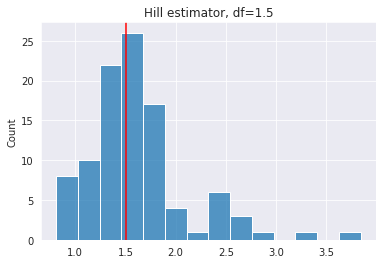
\includegraphics[width=0.6\textwidth]{Figures/hill.png}
    \caption{Hill estimator against $\nu=1.5$ StudentT}
    \label{fig:hill}
\end{figure}

Directly optimizing $\nu$ in the variational ELBO results in a trade-off between
accurate tail behaviour and matching the distribution around the mode.

For $x, y$ large:
\begin{align*}
    \Pr[X > x]             & \sim x^{-\alpha}                                       \\
    p(x)                   & \sim \alpha x^{-\alpha - 1}                            \\
    \log p(x)              & \sim \log \alpha - (\alpha + 1) \log x                 \\
    \log \frac{p(x)}{p(y)} & \sim (\alpha + 1) \log \frac{y}{x}                     \\
    \alpha                 & \sim \frac{\log p(x) - \log p(y)}{\log y - \log x} - 1
\end{align*}
Note that $p$ can be unnormalized as the partition function is cancelled out.
For example. setting $x=10$ and $y=20$ yields an estimate of $1.4799$
for a $\nu=1.5$ StudentT.

\feynman{Consider Richardson extrapolation to accelerate this limit. Rate of convergece in limit must be a power}

\subsubsection{Approximate marginalization}

\feynman{Is this feasible for PP?}

\textbf{Problem}: Joint distributions (e.g. location-scale mixtures) require
marginalization before we can get $p(x)$.

\textbf{Our Method}: Approximate with discrete mixture
\begin{align*}
    p(x) = \int p(x|z) p(z) dz \approx \frac{1}{N} \sum_{i=1}^N p(x \mid z_i)\quad\text{where}~z_i\simiid p(z)
\end{align*}

\begin{figure}[H]
    \centering
    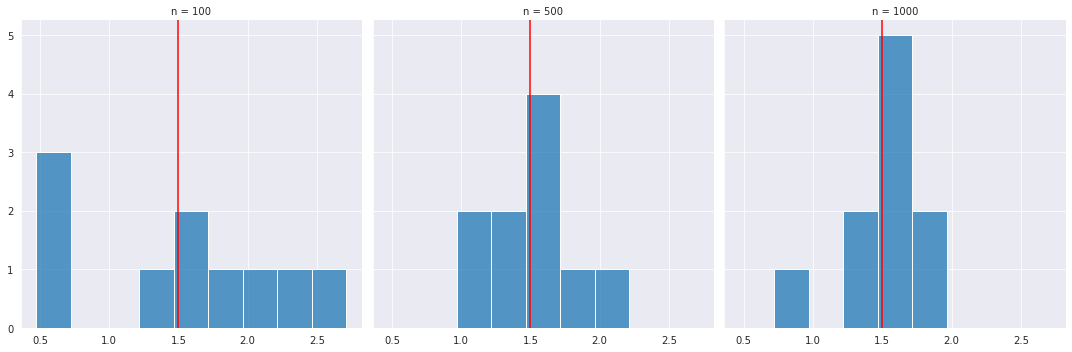
\includegraphics[width=0.9\textwidth]{Figures/our-estimator.png}
    \caption{Tail index estimation on location-scale mixture representation
        for StudentT, where the mixture is discretized to $n$ components.}
    \label{fig:approx_marg}
\end{figure}


\section{Experiments}

These experiments investigate the behavior of neural density estimators with
\emph{heavy-tailed base distribution}.
Specifically, we consider a masked autoregressive flow \cite{papamakarios2017masked}
transform of a generalized Student's t distribution as a density estimator $q_\theta(X)$
in a variational inference framework. To fit $q_\theta$ to a target distribution
$\pi$, the ELBO gradient is reparameterized and Monte-Carlo approximated
\begin{align*}
    \nabla_\theta \EE_{q_\theta} \log \frac{\pi(X)}{q_\theta(X)}
     & = \nabla_\theta \EE_p \log \frac{
        \pi(X)
    }{p_\theta(f_\theta^{-1}(X))
    \left\lvert \det \nabla f_\theta^{-1}(X) \right\rvert}    \\
     & = \EE_p \nabla_\theta \log \frac{
        \pi(X)
    }{p_\theta(f_\theta^{-1}(X))
    \left\lvert \det \nabla f_\theta^{-1}(X) \right\rvert}    \\
     & \approx \frac{1}{n} \sum_i^n \nabla_\theta \log \frac{
        \pi(x_i)
    }{p_\theta(f_\theta^{-1}(x_i))
        \left\lvert \det \nabla f_\theta^{-1}(x_i) \right\rvert}
\end{align*}

\feynman{Careful, $D_{KL}(N(0,1), \text{Cauchy}(0,1) \approx 0.2592 < \infty = D_{KL}(\text{Cauchy(0,1), N(0,1)})$}

\subsection{Applications in PPL inference}

The experiments in this section are conducted using the \texttt{beanmachine} PPL, where
inference is conducted following a Metropolis-within-Gibbs framework.

\subsection{Normal-normal location mixture}

We first consider a Normal-Normal conjugate inference problem where the posterior
is known to be a Normal distribution as well.
\Cref{fig:normal_normal} shows the resulting density approximation, which can
be seen to be reasonable for both a Normal base distribution (the ``correct'' one)
and a StudentT base distribution. This suggests that mis-specification (i.e. heavier
tails in the base distribution than the target) may not be too problematic.

\begin{figure}[H]
    \centering
    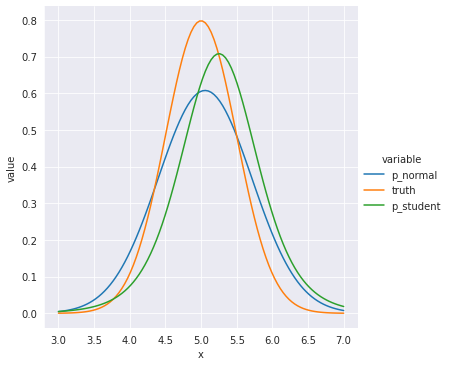
\includegraphics[width=0.6\textwidth]{Figures/normal_normal_posterior.png}
    \caption{VI against a Normal posterior}
    \label{fig:normal_normal}
\end{figure}

\subsection{StudentT scale mixture representation}

We next consider a heavy-tailed posterior target density by using a scale-mixture
representation for Student's t. Specifically, if $v \sim \chi_2(\nu)$
and $y \mid v \sim N(0, v)$ then the marginal distribution of $y$ is StudentT
with $\nu$ degrees of freedom.
In this experiment, we also allow the degrees of freedom for the base StudentT
distribution to be optimized as well in \texttt{p\_student\_df\_vi} and set
the degrees of freedom equal to the true $\nu$ in \texttt{p\_student\_vi}.
While using the true $\nu$ does yield an almost exact fit, optimizing $\nu$ is
more practical.

\begin{figure}[H]
    \centering
    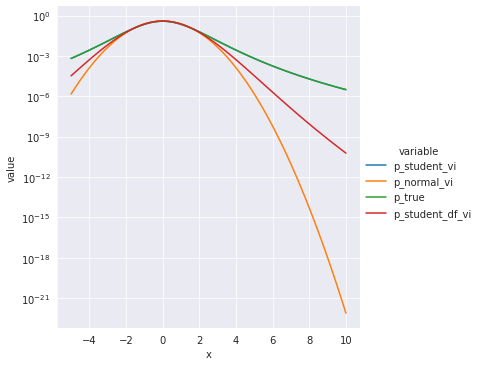
\includegraphics[width=0.6\textwidth]{Figures/studentt_log_scale.png}
    \caption{VI against StudentT represented by a Normal scale mixture}
    \label{fig:studentt_loc_scale}
\end{figure}

\subsection{Bayesian Robust Regression}

$n = 100$, $d = 10$.

$X_{ij} \simiid N(0,1)$ for $i \in [n]$, $j \in [d]$.

$y_i \simiid \text{StudentT}(\text{loc}=X \beta, df=5)$

Improper ``flat'' prior on $\beta$ to ensure heavy-tailed posterior.

\begin{figure}[H]
    \centering
    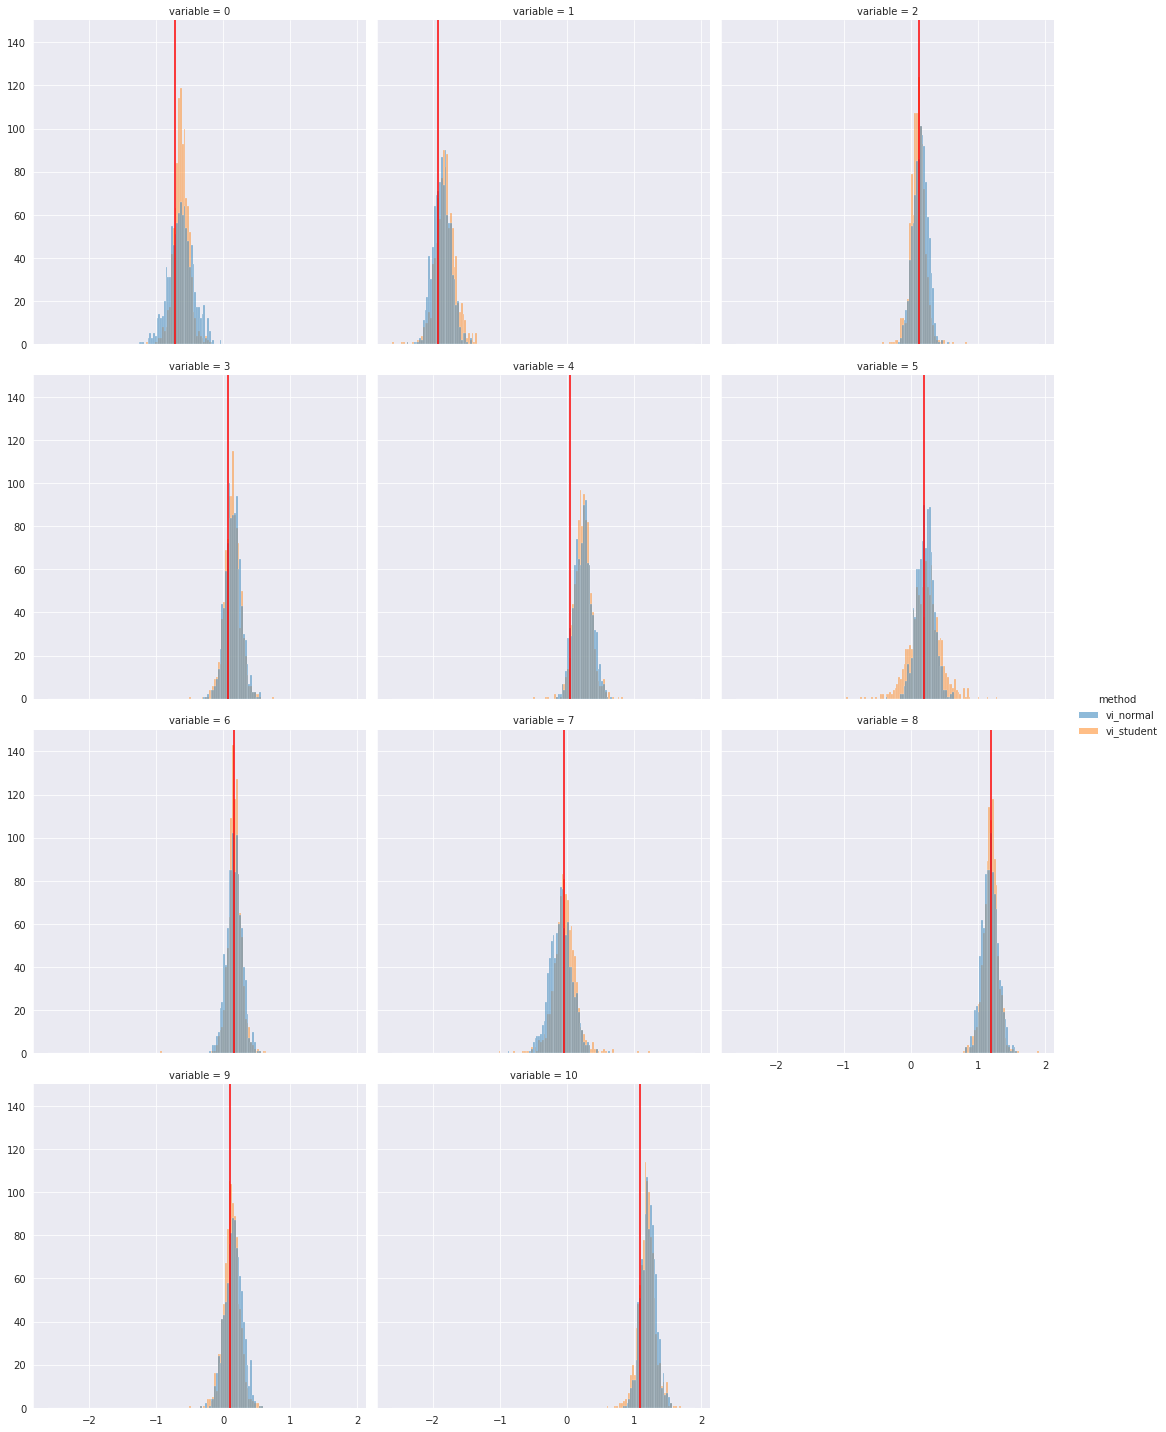
\includegraphics[width=0.6\textwidth]{Figures/blr.png}
    \caption{VI of Bayesian robust linear regression}
    \label{fig:blr}
\end{figure}

\feynman{Can work out the exponent with asymptotic approximations; compare?}

\subsection{Eight schools}

\begin{figure}[H]
    \centering
    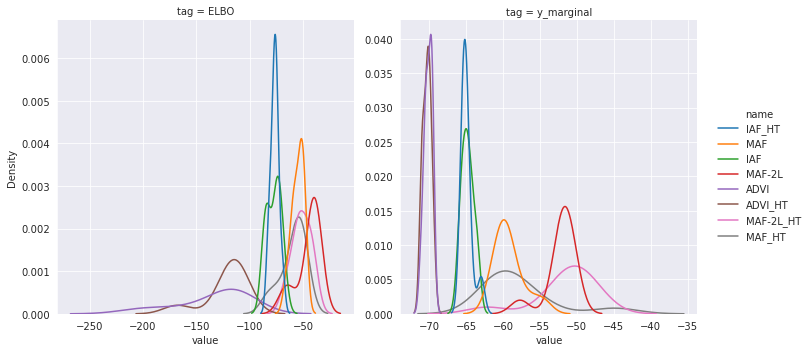
\includegraphics[width=0.8\textwidth]{Figures/eight_schools.png}
    \begin{tabular}{rcc}
        \toprule
                  & ELBO                & $\log P(y)$       \\
        \midrule
        ADVI      & -193.86 $\pm$ 33.50 & -70.11 $\pm$ 0.52 \\
        ADVI-HT   & -121.54 $\pm$ 19.59 & -70.29 $\pm$ 0.54 \\
        MAF       & -55.06 $\pm$ 5.46   & -59.14 $\pm$ 1.99 \\
        MAF-HT    & -59.63 $\pm$ 6.74   & -57.84 $\pm$ 4.97 \\
        MAF-2L    & -45.01 $\pm$ 11.02  & -52.19 $\pm$ 2.06 \\
        MAF-2L-HT & -51.67 $\pm$ 8.72   & -51.53 $\pm$ 4.23 \\
        IAF       & -77.67 $\pm$ 6.47   & -64.79 $\pm$ 0.80 \\
        IAF-HT    & -76.67 $\pm$ 3.71   & -64.91 $\pm$ 0.76 \\
        \bottomrule
    \end{tabular}
    \caption{Final ELBO and (MC estimate of) log marginal $\log P(y)$ after 5000 steps}
    \label{fig:blr}
\end{figure}



\subsection{Importance weights}

When the importance sampling density is more peaked than the target density.

\cite{wang2018variational} example 3.1: Let $p = N(0, \sigma_p^2)$, $q = N(0, \sigma_q^2)$,
and for $x \sim q$ let $w(x) = \frac{p(x)}{q(x)}$. If $\sigma_p > \sigma_q$,
then $w$ has tail index $\frac{\sigma_p^2}{\sigma_p^2 - \sigma_q^2}$.
Otherwise, $w$ is not fat-tailed.

\feynman{TODO}

\subsection{Some HTVAE example reconstructions and likelihoods}

\feynman{TODO. From \cite{sohn2015learning}, MNIST, Caltech-UCSD Birds, and Labeled Faces in the Wild.}

\section{Single-Site Normalizing Flow Variational Inference}


Let $\{q_\phi\}_{\phi \in \Phi}$ be a parameterized (variational) family.
Recall the variational ELBO
\begin{align*}
    \log p(y)
    = \log \int dx \frac{q_\phi(x)}{q_\phi(x)} p(x,y)
    \geq \int dx q_\phi(x) \log \frac{p(x,y)}{q_\phi(x)}
\end{align*}
The variational family's PDF $q_\phi(x)$ is assumed to be tractable, and
the joint PDF $p(x,y)$ may be obtained by running the probabilistic program forwards.
Finally, the Monte-Carlo method enables tractable approximation of the integral:
\begin{align*}
    \int dx q_\phi(x) \log \frac{p(x,y)}{q_\phi(x)}
     & \approx \log \frac{p(x,y)}{q_\phi(x)}\qquad x \sim q_\phi
\end{align*}
making the ELBO tractable.

Assume there are $d$ latent variables $x = (x_i)_{i=1}^d$.
Single-site variational inference (i.e.\ CaVI, coordinate-ascent variational
inference) sequentially iterates over $i \in [d]$, performing Monte-Carlo
\begin{align*}
    \phi \leftarrow
    \phi + \alpha_t \nabla_{\phi} \EE_{\setminus \{i\}} \EE_{i} q_\phi(x) \log \frac{p(x,y)}{q_\phi(x)}
\end{align*}

\todo{Finish description, vary the number of MC samples between two expectations}

\subsection{Cached Inverses}

The Monte-Carlo ELBO
\begin{align*}
    \sum_i \log p(x_i, y) - \log q(x_i) \qquad x_i \sim q
\end{align*}
requires both sampling and evaluating log densities with respect to $q$.
When $q$ is taken to be a distribution parameterized by a normalizing flow
$q(x) = \lvert \frac{df}{dx} \rvert p(f^{-1}(x))$, log density evaluations
require evaluating the inverse flow $f^{-1}$ whereas sampling involves
pushing forward samples $x \sim p$ along the flow's forward direction.

Modern normalizing flow architectures typically
are much more expensive to compute in one direction (c.f. IAF vs MAF), with
some flows (NAF, SoS, ResidualFlows) requiring an optimization to approximate
the inverse flows. To circumvent this problem, we identify a critical optimization
for VI that caching can be used to avoid flow inversion during Monte-Carlo training.
That is, by caching pairs $(x_i, y_i = f(x_i))$ sampled during MC ELBO,
the entropy term $\log q(y_i) = \log \lvert \frac{df}{dx}(x_i) \rvert + \log p(x_i)$
can be evaluated without explicit inversion.

\todo{Run-time comparisons for ELBO with/without caching}

\subsection{NaMI structured conditional flows}

The NaMI algorithm \cite{webb2017faithful} can be used for model inversion, enabling
single-site flow distributions which depend on the values of adjacent nodes (as well as
amortized variational inference where the variational families $q_{(\phi,y)}(x)$
depend on the conditioned observations $y$.


\section{Meeting Notes}

\begin{enumerate}
    \item We added a knob for heavy tail, how do we make fair comparison? Increase the flexibility of the flow for non-Gaussian.
    \item Neural network weights heavy tailed; can we learn VI with heavy-tailed distributions.
\end{enumerate}

\section{Discussion}

Limitations: only considered symmetric base distributions, could also consider skewness \citep{gupta2003multivariate}.

\bibliography{refs_ftvi}

\end{document}